\setlength{\parskip}{\baselineskip}
\section[Theoretical Modeling]{Theoretical Modeling \& Robustness Analysis}

\begin{frame}
	\huge Theoretical Modeling \& Robustness Analysis
\end{frame}

\begin{frame}{PyTorch, C/C++, MATLAB}
	\begin{itemize}
		\item
	\end{itemize}
\end{frame}

\begin{frame}{Algorithms}
	\begin{itemize}
		\item
	\end{itemize}
\end{frame}

\begin{frame}{Memory Footprint: AlexNet Parameters}
	\begin{table}[H]
		\centering
		\begin{tabular}{llll}
			\toprule
			\textbf{Layer} & \textbf{\#Parameters}        & \textbf{Footprint} & \textbf{Memory (\%)} \\
			\midrule
			Conv1          & $64 * 3 * 11 * 11 = 23232$   & 92.92KB            & 0.04                 \\
			Conv2          & $192 * 64 * 5 * 5 = 307200$  & 1.22MB             & 0.5                  \\
			Conv3          & $384 * 192 * 3 * 3 = 663552$ & 2.65MB             & 1.09                 \\
			Conv4          & $256 * 384 * 3 * 3 = 884736$ & 3.53MB             & 1.45                 \\
			Conv5          & $256 * 256 * 3 * 3 = 589824$ & 2.35MB             & 0.97                 \\
			FC1            & $9216 * 4096 = 37748736$     & 150.99MB           & 61.79                \\
			FC2            & $4096 * 4096 = 16777216$     & 67.10MB            & 27.46                \\
			FC3            & $4096 * 1000 = 4096000$      & 16.38MB            & 6.70                 \\
			\midrule
			\textbf{Total} & 61090496                     & 244.36MB           & 100                  \\
			\bottomrule
		\end{tabular}
	\end{table}
\end{frame}

\begin{frame}{Memory Footprint: AlexNet Data Stages}
	\begin{table}[H]
		\small
		\centering
		\scalebox{0.9}{
			\begin{tabular}{llll}
				\toprule
				\textbf{Layer} & \textbf{\#Data}          & \textbf{Footprint} & \textbf{Memory (\%)} \\
				\midrule
				Image          & $3 * 224 * 224 = 150528$ & 150.52KB           & 6.07                 \\
				Conv1          & $64 * 55 * 55 = 193600$  & 774.40KB           & 31.22                \\
				MaxPool1       & $64 * 27 * 27 = 46656$   & 186.62KB           & 7.52                 \\
				Conv2          & $192 * 27 * 27 = 139968$ & 559.87KB           & 22.57                \\
				MaxPool2       & $192 * 13 * 13 = 32448$  & 129.79KB           & 5.23                 \\
				Conv3          & $384 * 13 * 13 = 64896$  & 259.58KB           & 10.46                \\
				Conv4          & $256 * 13 * 13 = 43264$  & 173.05KB           & 6.98                 \\
				Conv5          & $256 * 13 * 13 = 43264$  & 173.05KB           & 6.98                 \\
				MaxPool3       & $9216$                   & 36.86KB            & 1.49                 \\
				FC1            & $4096$                   & 16.38KB            & 0.66                 \\
				FC2            & $4096$                   & 16.38KB            & 0.66                 \\
				FC3            & $1000$                   & 4KB                & 0.16                 \\
				\midrule
				\textbf{Total} & 682856                   & 2.48MB             & 100                  \\
				\bottomrule
			\end{tabular}
		}
	\end{table}
\end{frame}

\begin{frame}{Memory Footprint Reduction}
	\begin{itemize}
		\item
	\end{itemize}
\end{frame}

\begin{frame}{Memory Footprint Reduction: Evaluation}
	\begin{itemize}
		\item
	\end{itemize}
\end{frame}

\begin{frame}{Memory Footprint Reduction: Floating Point}
	\begin{table}[H]
		\centering
		\begin{tabular}{p{2cm} p{2cm} p{3cm} p{3cm}}
			\toprule
			\textbf{Tool} & \textbf{Data type} & \textbf{Top-1 Error rate (\%)} & \textbf{Avg. inference time (sec)} \\
			\midrule
			PyTorch       & float64            & 0                              & 0.091                              \\
			PyTorch       & float32            & 0                              & 0.034                              \\
			MATLAB        & float64            & 0                              & 6.624                              \\
			MATLAB        & float32            & 0                              & 8.162                              \\
			MATLAB        & float16            & 0.36                           & 147.480                            \\
			\bottomrule
		\end{tabular}
	\end{table}
\end{frame}

\begin{frame}{Memory Footprint Reduction: Fixed Point}
	\begin{table}[H]
		\centering
		\begin{tabular}{p{2cm} p{2cm} p{3cm} p{3cm}}
			\toprule
			\textbf{Tool} & \textbf{Data type} & \textbf{Top-1 Error rate (\%)} & \textbf{Avg. inference time (sec)} \\
			MATLAB        & fixed64            & 0                              & 7.318                              \\
			MATLAB        & fixed32            & 0                              & 7.692                              \\
			MATLAB        & fixed16            & 22                             & 6.650                              \\
			MATLAB        & fixed14            & 28.44                          & 6.813                              \\
			MATLAB        & fixed12            & 36.24                          & 6.797                              \\
			MATLAB        & fixed10            & 77.07                          & 6.929                              \\
			MATLAB        & fixed8             & 100                            & 6.312                              \\
			\bottomrule
		\end{tabular}
	\end{table}
\end{frame}

\begin{frame}{Memory Footprint Reduction: Fixed Point MQE}
	\begin{table}[H]
		\centering
		\begin{tabular}{lll}
			\toprule
			\textbf{Tool} & \textbf{Data type} & \textbf{Top-1 Error rate (\%)}\\
			\midrule
				MATLAB 	& fixed64	& 0 	\\
				MATLAB 	& fixed32	& 0 	\\
				MATLAB 	& fixed16	& 4.42 	\\
				MATLAB 	& fixed14	& 17.59 \\
				MATLAB 	& fixed12	& 48.11 \\
				MATLAB 	& fixed10	& 86.91	\\
				MATLAB 	& fixed8	& 99.3 	\\
			\bottomrule
		\end{tabular}
	\end{table}
\end{frame}

\begin{frame}{Memory Footprint Reduction: All data types tested}
	\centering
	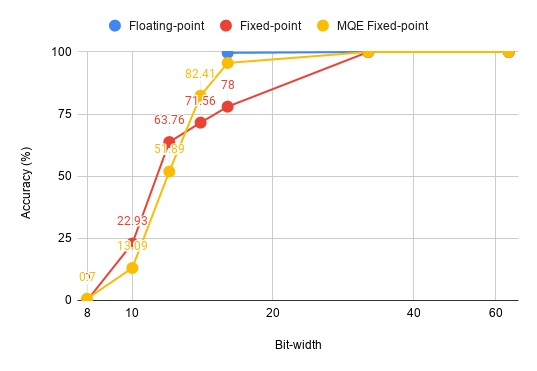
\includegraphics[width=0.7\textwidth]{../Images/Weights-distributions/data-types-accuracy-chart.png}\\
\end{frame}
